\documentclass[xcolor=table,usenames,dvipsnames]{beamer}

\usepackage[british]{babel}
\usepackage{courier}
\usepackage{xcolor}
\usepackage{mdframed}
\usepackage[utf8]{inputenc}
\usepackage{multicol,calc}
\usepackage{ragged2e} 
\usepackage{menukeys}
\usepackage{graphicx}
\usepackage{url}
\usepackage{amsmath, amsthm, amssymb}
\usepackage{setspace} %espaciado
\usepackage{etoolbox} %color bibliografía
\usepackage{wrapfig} %imagen alrededor texto
\usepackage{ajustes}



\title[Modulación Digital con SDR]{
	Modulación Digital con SDR}

\author[Ingeniería Electrónica]{Creación Colectiva\\
	\tiny 
	IPA2020\\
	Riaño Walter, Barragan Wilmar,Montana Camilo, Giraldo Martin, Alfonso Andres, Hellcenk Murillo, Cifuentes Jorge, Lizcano Gonzalo, Marín Laura, Torres Omar, Guayara Camila, Firigua Lorena\\
	\scriptsize
	Tutor\\ Rodríguez Mújica Leonardo}

\institute[Universidad de Cundinamarca]{
	Facultad de Ingeniería\\
	Universidad de Cundinamarca}

\date{2020}

%-----------------------------------

\begin{document}
	
	%espaciado item
	\let\olditemize\itemize
	\def\itemize{\olditemize\itemsep=4pt }
	\footnotesize
	
	\begin{frame}
	\titlepage
\end{frame}
%-----------------------------------

\begin{frame}
\frametitle{Contenidos generales}
\tableofcontents[subsectionstyle=hide/hide, subsubsectionstyle=hide/hide]
\end{frame}
%-----------------------------------


%-----------------------------------

%\input{parte1/SDR-I}

%/////////////////////////

%\input{parte2/SDR-II}

%/////////////////////////

%\input{parte3/SDR-III}

%/////////////////////////

\section{LABORATORIOS MODULACIONES DIGITALES}
\begin{frame}

\pgfdeclareimage[width=\paperwidth,height=\paperheight]{bg}{imagenes/fondo_seccion}
\setbeamertemplate{background}{\pgfuseimage{bg}}

\definecolor{greenU}{RGB}{212,202,72}
\setbeamercolor{block body}{fg=Black,bg=greenU}
\begin{block}{}
\centering
\vspace{8mm}
\Large{LABORATORIOS MODULACIONES DIGITALES}
\vspace{8mm}
\end{block}
\end{frame}
%-----------------------

{
\begin{frame}
\frametitle{Parte IV - Tabla de contenidos}
\begin{spacing}{1.5}
\tableofcontents[currentsection,sectionstyle=hide/hide,subsectionstyle=show/show/hide, subsubsectionstyle=hide]
\end{spacing}
\end{frame}
}

%///////////////////////////////////////////////////////////////
\subsection{Lab17: BPSK}

%*********************
\begin{frame}{}

\pgfdeclareimage[width=\paperwidth,height=\paperheight]{bg}{imagenes/fondo_lab}
\setbeamertemplate{background}{\pgfuseimage{bg}}

\bfseries{\textrm{\LARGE Lab17\\ \Large BPSK}}
\raggedright
\end{frame}
%*************
%----------------------------------------
\begin{frame}

\pgfdeclareimage[width=\paperwidth,height=\paperheight]{bg}{imagenes/fondo3}
\setbeamertemplate{background}{\pgfuseimage{bg}}

\frametitle{\underline{\textbf{Modulación BPSK}}}

Para obtener una señal modulada se utiliza un modulador balanceado (Modulador de producto) que funciona como un conmutador, ya que a medida que la señal de información muestre un “1” o un “0” la portadora conmuta en dos fases diferentes. En un modulador BPSK se asigna +1 V al 1 lógico y -1 V al 0 lógico, la portadora de entrada, $\sin\omega_{c}t$se multiplica por +1 o por -1. En consecuencia, la señal de salida puede ser +1 $\sin\omega_{c}t$ o 1 $\sin\omega_{c}t$; el primer producto representa una señal que está en fase con el oscilador de referencia, y el último producto, una señal que está desfasada 180 grados [11]\\
La ecuación de salida de un modulador BPSK es proporcional a:\\

$$y(t)=[\sin(2 \pi f_{a}t)]X[\sin(2 \pi f_{c}t)]$$\\

\begin{enumerate}			
	\item{$f_{a}$: frecuencia fundamental máxima de la entrada binaria (señal moduladora) en hertz.}\\
	\item{$f_{c}$: frecuencia de portadora de referencia en hertz.}\\
\end{enumerate}
\end{frame}
%-----------------------------------------
\begin{frame}{Modulador BPSK en GRC}
\begin{figure}[H]
\vspace{-3mm}
\centering
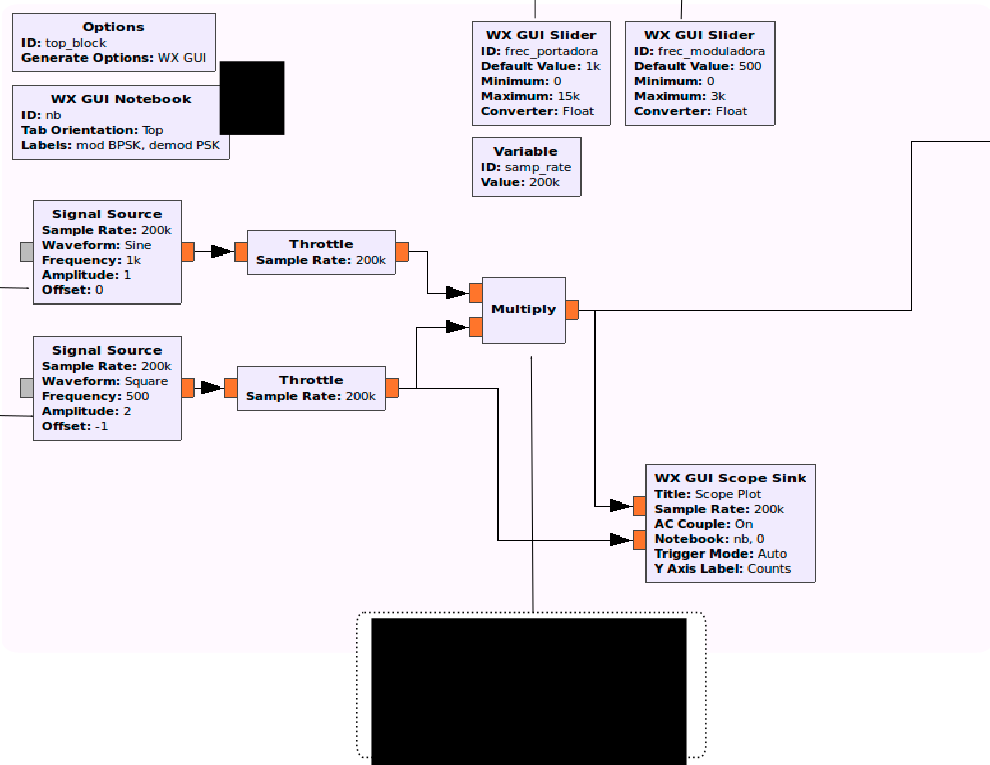
\includegraphics[width=0.9\textwidth]{Modulaciones_digitales/lab17/pdf/PSK_2.pdf}
\end{figure}
\end{frame}
%----------------------------------------
\begin{frame}{Modulación BPSK}
\begin{figure}[H]
\vspace{-3mm}
\centering
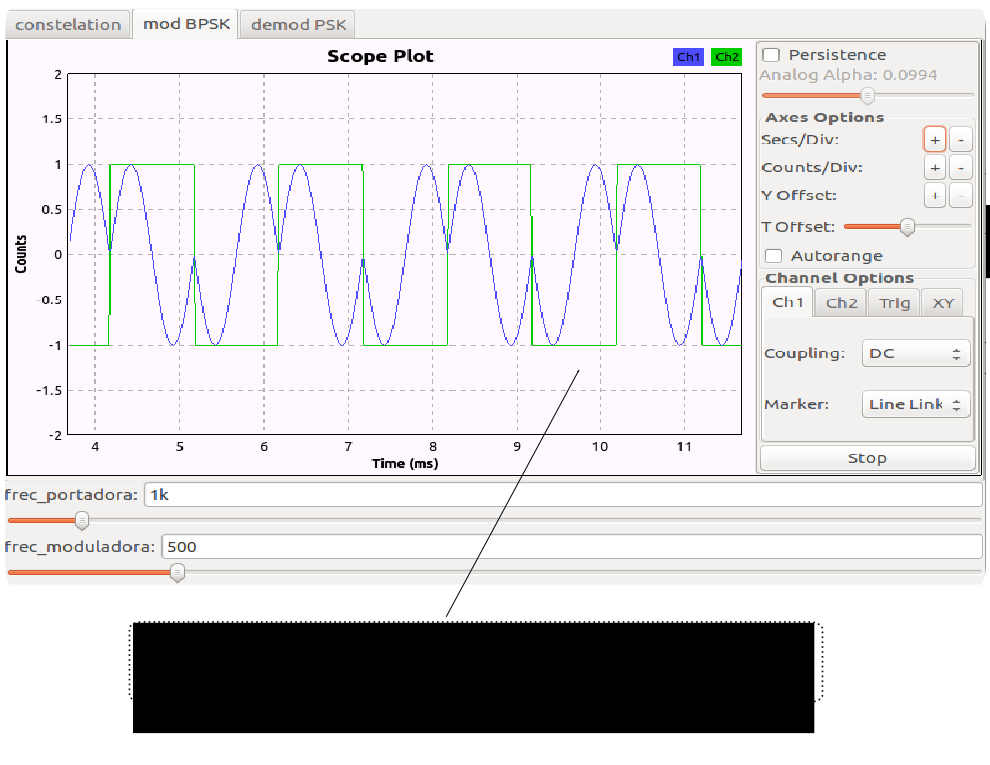
\includegraphics[width=0.9\textwidth]{Modulaciones_digitales/lab17/pdf/PSK_3.pdf}
\end{figure}
\end{frame}
%----------------------------------------
\begin{frame}

\pgfdeclareimage[width=\paperwidth,height=\paperheight]{bg}{imagenes/fondo3}
\setbeamertemplate{background}{\pgfuseimage{bg}}

\frametitle{\underline{\textbf{Demodulación BPSK}}}

El circuito de recuperación coherente de portadora detecta y regenera una señal de portadora que es coherente, tanto en fase como en frecuencia, con la portadora original de transmisión. El modulador balanceado es un detector de producto; la salida es el producto de las dos entradas (la señal BPSK y la portadora recuperada).El filtro pasabajas (LPF) separa los datos binarios recuperados de la señal demodulada.[11]

\end{frame}
%-----------------------------------------
\begin{frame}{Demodulador BPSK en GRC}
\begin{figure}[H]
\vspace{-3mm}
\centering
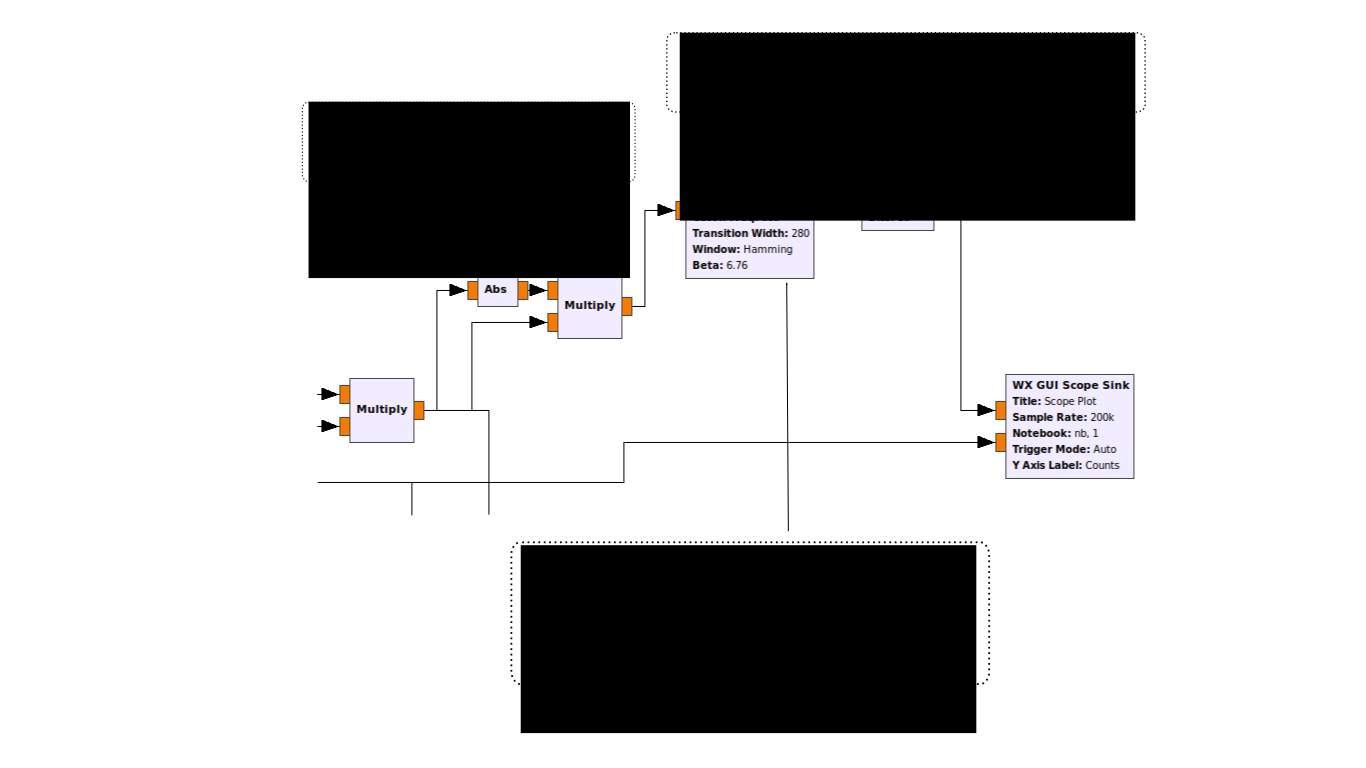
\includegraphics[width=0.8\textwidth]{Modulaciones_digitales/lab17/pdf/PSK_4.pdf}
\end{figure}
\end{frame}
%----------------------
\begin{frame}{Demodulación BPSK}
\begin{figure}[H]
\vspace{-3mm}
\centering
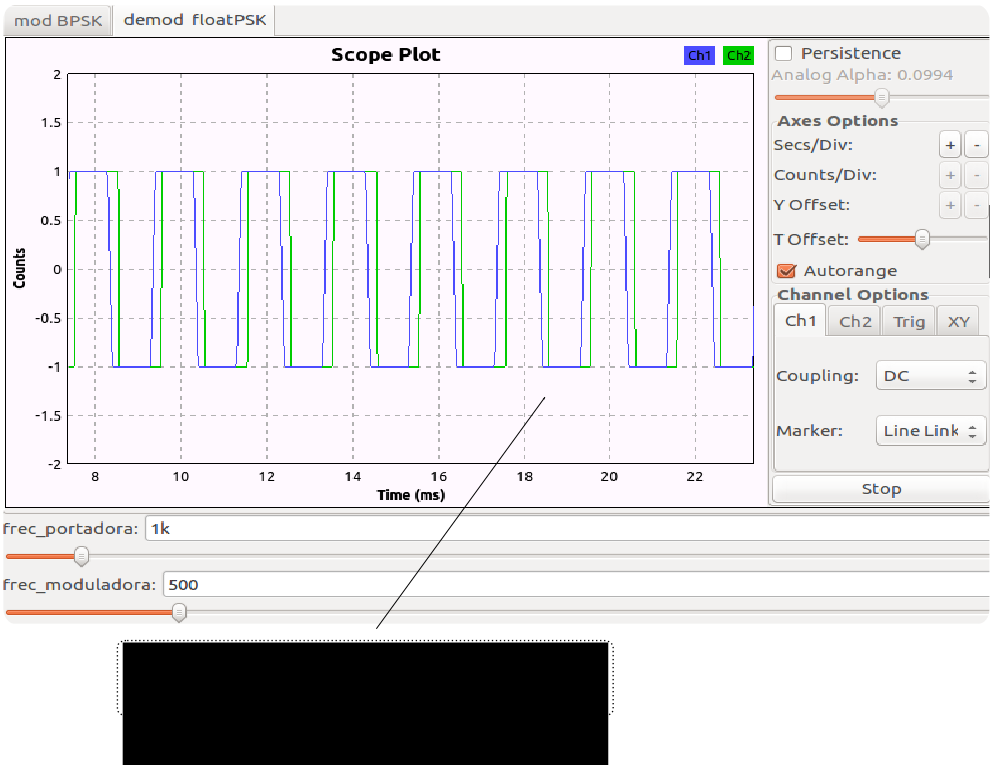
\includegraphics[width=0.9\textwidth]{Modulaciones_digitales/lab17/pdf/PSK_5.pdf}
\end{figure}
\end{frame}
\subsection{Lab18: Esquema de la Modulación y Demodulación DPSK en GNU Radio}
%*********************
\begin{frame}{}

\pgfdeclareimage[width=\paperwidth,height=\paperheight]{bg}{imagenes/fondo_lab}
\setbeamertemplate{background}{\pgfuseimage{bg}}

\bfseries{\textrm{ \Large Lab 18: \\Esquema de la Modulación y \\Demodulación DPSK \\en GNU Radio}}
\raggedright
\end{frame}
%********************

\begin{frame}{Esquema de la Modulación y Demodulación DPSK en GNU Radio}

\pgfdeclareimage[width=\paperwidth,height=\paperheight]{bg}{imagenes/fondo3}
\setbeamertemplate{background}{\pgfuseimage{bg}}

\begin{figure}[H]
	\vspace{-3mm}
	\centering
	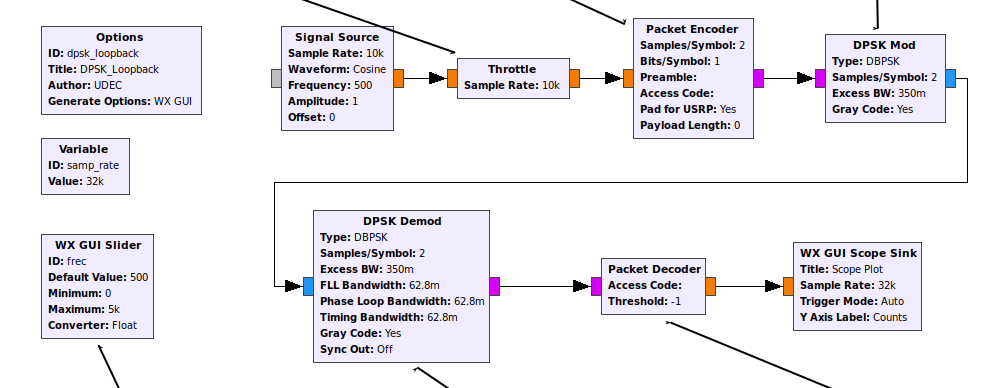
\includegraphics[width=0.9\textwidth]{Modulaciones_digitales/lab18/pdf/01Inicio.pdf}
\end{figure}
\end{frame}

	\begin{frame}
	\frametitle{\underline{\textbf{Objetivo de la guía del ejemplo Modulación DPSK}}}	
	Comprender el funcionamiento de los bloques de modulación y modulación DPSK, así como los bloques Packet Encoder y Packet decoder mediante la codificación y modulación de una señal, para luego recuperar la señal mediante la decodificación y modulación y finalmente ser vista en el ventana grafica WX GUI Scope Sink..\vspace{2mm}
	\end{frame}

	\begin{frame}
	\begin{enumerate}[1.]
	\frametitle{\underline{\textbf{Guía Ejemplo Modulación DPSK}}}
	\item{Modulador DPSK: En un modulador Dpsk, se realiza una operación XNOR entre el bit actual de la señal digital de información y bit transmitido con anterioridad. La salida de esta operación entra en un modulador PSK. En el modulador PSK, siempre que la salda de la puerta XNOR aparezca un 1 lógico, el modulador producira una salida analógica $+Cos(Wct)$. Si en lugar de esto la salida de la XNOR es un 0 lógico, en el modulador aparecerá la señal de salida $-Cos(Wct)$. Es decir, la salida de XNOR va a cambiar de valor cada vez que aparezca un 0 lógico en la señal digital de entrada al modulador, y por consiguiente producirá un cambio de fase analógica de salida.}\\

	\end{enumerate}
	\end{frame}	
	
	\begin{frame}
	\begin{enumerate}[1.]
	\frametitle{\underline{\textbf{Guía Ejemplo Modulación DPSK}}}
	\item{Demodulador DPSK: Es un circuito bastante simple que solo necesita un multiplicador analógico, un latch de retraso de 1 bit y un filtro pasa bajas con frecuencia de corte menor que $2Wc$. Cada vez que la salida del multiplicador es $Wct$, es decir se ha producido un cambio de fase entre la señal de entrada y señal anterior retrasada , a la salida del filtro pasa bajas aparece un 0 lógico, que es precisamente en lo que consiste la modulación DPSK. En caso contrario, si no se produce un cambio de fase la salida del filtro es un 1 lógico.}\\

	\end{enumerate}
	\end{frame}
	
	\begin{frame}
	\begin{enumerate}[1.]
	\frametitle{\underline{\textbf{Codificación y Modulación DPSK}}}
	\item{Packet Encoder: Empaqueta los bytes de una longitud y carga determinada con un encabezado, código de acceso y preámbulo.  El encabezado es un repetición 2x de la longitud de la carga útil (16 bits para cada campo).}\\
	\item{DPSK Mod este bloque modulador DPSK recibe en su entrada una secuencia de de bytes  (carácter sin signo) y en su salida entrega la señal modulada en banda base.}\\
	\end{enumerate}
	\end{frame}

\begin{frame}{Packet Encoder y DPSK Mod}
\begin{figure}[H]
	\vspace{-3mm}
	\centering
	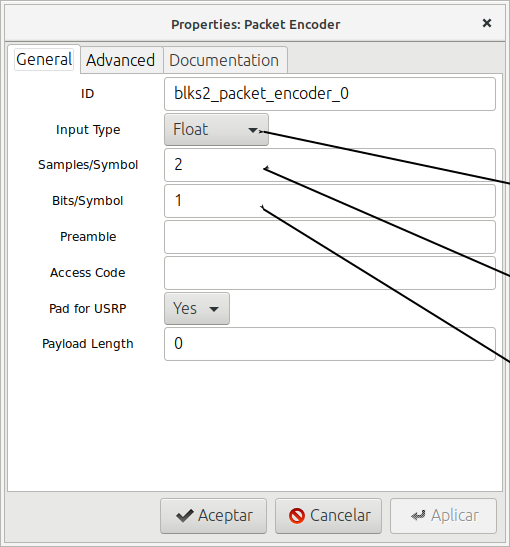
\includegraphics[width=0.9\textwidth]{Modulaciones_digitales/lab18/pdf/02Packet_Encoder.pdf}
\end{figure}
\end{frame}

\begin{frame}{Packet Encoder y DPSK Mod}
\begin{figure}[H]
	\vspace{-3mm}
	\centering
	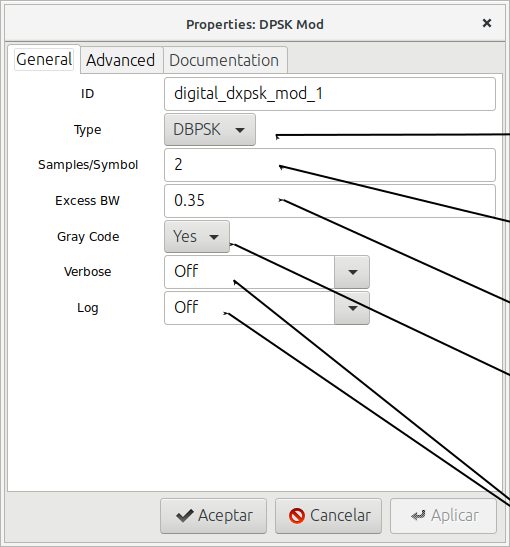
\includegraphics[width=0.9\textwidth]{Modulaciones_digitales/lab18/pdf/03DPSK_Mod.pdf}
\end{figure}
\end{frame}

	\begin{frame}
	\begin{enumerate}[1.]
	\frametitle{\underline{\textbf{Demodulación y Decodificación DPSK}}}
	\item{DPSK Demod: 
Realiza la demodulación de la señal compleja modulada en la frecuencia de banda base y entrega en su salida un flujo de bytes empaquetados }\\
	\item{Packet Decoder: El decodificador busca el código de  con el numero de bit disponibles incorrecto, cuando lo encuentra , lee el encabezado para obtener la longitud de la carga útil extraerla y generar la carga útil de bit original.}\\
	\end{enumerate}
	\end{frame}
	
\begin{frame}{DPSK Demod y Packet Decoder }
\begin{figure}[H]
	\vspace{-3mm}
	\centering
	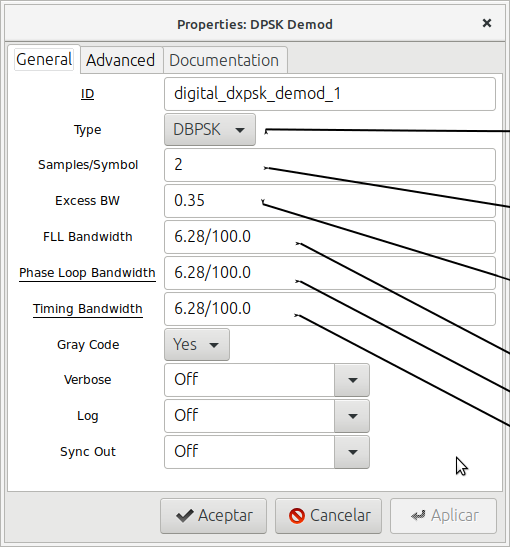
\includegraphics[width=0.9\textwidth]{Modulaciones_digitales/lab18/pdf/04DPSK_Demod.pdf}
\end{figure}
\end{frame}

\begin{frame}{DPSK Demod y Packet Decoder}
\begin{figure}[H]
	\vspace{-3mm}
	\centering
	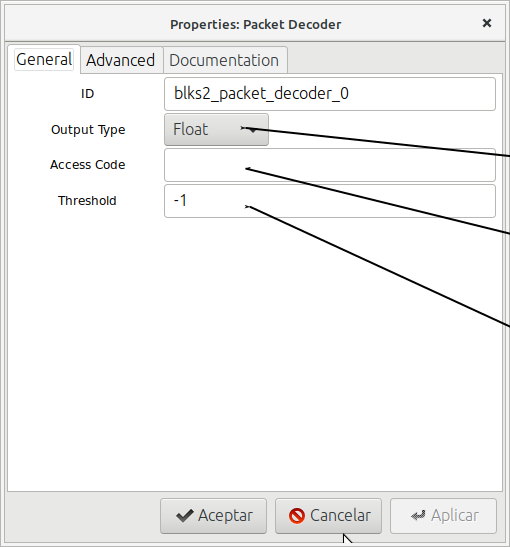
\includegraphics[width=0.9\textwidth]{Modulaciones_digitales/lab18/pdf/05Packet_Decoder.pdf}
\end{figure}
\end{frame}

\begin{frame}{ Señal Demodulada DPSK}
\begin{figure}[H]
	\vspace{-3mm}
	\centering
	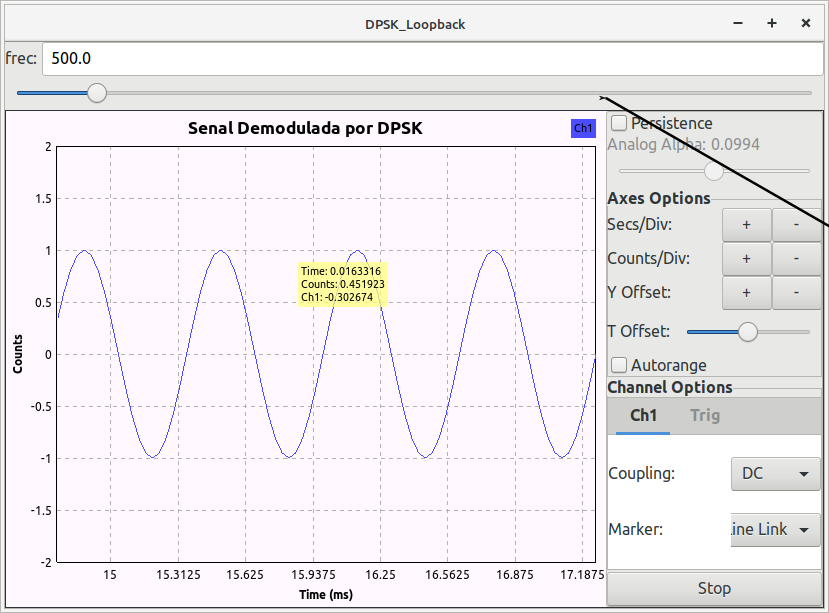
\includegraphics[width=0.9\textwidth]{Modulaciones_digitales/lab18/pdf/06Salida.pdf}
\end{figure}
\end{frame}
		


%\begin{frame}{Primeros pasos }
%\begin{figure}[H]
%	\vspace{-3mm}
%	\centering
%	\includegraphics[width=0.9\textwidth]{Actividades2/pdf/lab1_1.pdf}
%\end{figure}
%\end{frame}
\subsection{Lab19: Modulación QPSK en GRC}

%*********************
\begin{frame}{}

\pgfdeclareimage[width=\paperwidth,height=\paperheight]{bg}{imagenes/fondo_lab}
\setbeamertemplate{background}{\pgfuseimage{bg}}

\bfseries{\textrm{ \Large Lab 19: \\Modulación QPSK en GRC}}
\raggedright
\end{frame}
%********************

%--------------------------------------------------------------------------------------------
\begin{frame}{Modulación QPSK en GRC}

\pgfdeclareimage[width=\paperwidth,height=\paperheight]{bg}{imagenes/fondo3}
\setbeamertemplate{background}{\pgfuseimage{bg}}

\justifying
Este ejercicio mostrará la modulación digital QPSK en GRC donde los datos a enviar serán generados por el bloque Random Source el cual proveerá diferentes valores de manera aleatoria en el rango de 0 a 100, estos datos serán entregados en forma de bytes,para poderlos visualizar en un osciloscopio\cite{Universidad Militar Nueva Granada}

\end{frame}
%---------------------------------------------------------------------------
%\includegraphics[scale=1]{../imagenes/descarga.jpeg} 
\begin{frame}{Modulación QPSK en GRC}
\begin{figure}
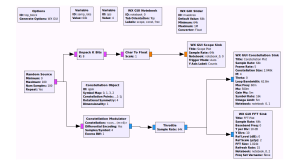
\includegraphics[scale=.4]{Modulaciones_digitales/lab19/pdf/lab19_1.pdf}
\end{figure}
\end{frame}
%--------------------------------------------------------------------------------------
\begin{frame}{Modulación QPSK en GRC}
\begin{figure}
\includegraphics[scale=.35]{Modulaciones_digitales/lab19/pdf/lab19_2.pdf}
\end{figure}
\end{frame}
%-----------------------------------------------------------------------------------
\begin{frame}{Modulación QPSK en GRC}
Pulsos de señal generados por Random Source
\begin{figure}
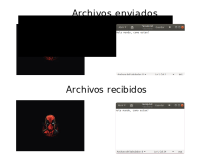
\includegraphics[scale=.4]{Modulaciones_digitales/lab19/pdf/lab19_3.pdf}
\end{figure}
\end{frame}
%---------------------------------------------------------------------------------------

\begin{frame}{Modulación QPSK en GRC}
\justifying
La definición de la constelación en el bloque Constellation Object se efectua de acuerdo a la cantidad de símbolos posibles en la misma dentro del espacio complejo o el diagrama de constelación. Para la constelación de QPSK se manejan 4 símbolos, entonces de acuerdo a la siguiente ecuación los bits para cada símbolo serían 2.\\
\centering
$\log_{2}(4)=2$ bits/símbolo\\
\end{frame}

%--------------------------------------------------------------------------------

\begin{frame}{Modulación QPSK en GRC}
\begin{figure}
\includegraphics[scale=.4]{Modulaciones_digitales/lab19/pdf/lab19_4.pdf}
\end{figure}
\end{frame}
%-----------------------------------------------------------------------------------

%---------------------------------------------------------------------------------------
\begin{frame}{Modulación QPSK en GRC}
\justifying
En el bloque Constellation modulator es posible implementar codificación diferencial con tan sólo habilitar este parámetro dentro de la configuración. La codificación diferencial o modulación diferencial en fase, no siempre asigna una fase determinada a cada símbolo (0 o 1), sino que de acuerdo a cada transición de bit, el modulador efectúa un cambio de fase de la siguiente manera:\\
\begin{itemize}
\item Si el siguiente símbolo es un 1 el cambio de fase es de $270^{\circ}$  
\item Si el siguiente símbolo es un 1 el cambio de fase es de $90^{\circ}$
\end{itemize}
La codificación diferencial contribuye a la reducción de errores y hace la modulación QPSK más robusta frente a la sensibilidad de ruido debido a los saltos de fase, puesto que no es necesario una demodulación síncrona con la portadora.\cite{Universidad Militar Nueva Granada}
\end{frame}

%---------------------------------------------------------------------------
\begin{frame}{Modulación QPSK en GRC}
\justifying
Constelación QPSK con codificación diferencial habilitada y 4 Muestras por símbolo
\begin{figure}
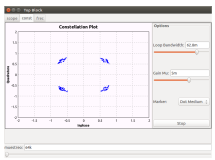
\includegraphics[scale=.4]{Modulaciones_digitales/lab19/pdf/lab19_5.pdf}
\end{figure}
\end{frame}
%-------------------------------------------------------------------------------------------
%\begin{frame}{Modulación QPSK en GRC}
%\begin{figure}
%\includegraphics[width=.9\textwidth]{parte1/QPSK/pdf/QPSK_6.pdf}
%\end{figure}
%\end{frame}
%------------------------------------------------------------------------------------------
\begin{frame}{Modulación QPSK en GRC}
Espectro de señal QPSK modulada a una frecuencia de muestreo igual a 64 kHz
\begin{figure}
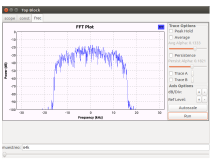
\includegraphics[width=.8\textwidth]{Modulaciones_digitales/lab19/pdf/lab19_7.pdf}
\end{figure}
\end{frame}

\subsection{Lab20:Modulacion digital QAM}

%*********************
\begin{frame}{}

\pgfdeclareimage[width=\paperwidth,height=\paperheight]{bg}{imagenes/fondo_lab}
\setbeamertemplate{background}{\pgfuseimage{bg}}

\bfseries{\textrm{\LARGE Lab20\\ \Large Modulacion QAM}}
\raggedright
\end{frame}
%*********************

\begin{frame}{Modulacion de amplitud en cuadratura QAM}
\begin{flushleft}
La modulación de amplitud en cuadratura, en inglés Quadrature Amplitude Modulation (QAM), es una técnica de modulación digital avanzada que transporta datos, técnica en la cual la informacion va a ser modulada tanto en amplitud como en fase (la señal de portadora va a ser modificada en amplitud y fase) o sea que la informacion digital está contenida, tanto en la amplitud como en la fase de la portadora trasmitida. Esto se consigue modulando una misma portadora, desfasando 90º la fase y la amplitud.
\end{flushleft}

La modulación QAM, es una forma de modulación digital en donde la información digital está contenida, tanto en la amplitud como en la fase de la portadora trasmitida.
\end{frame}
%*********************

\begin{frame}{Modulacion de amplitud en cuadratura QAM}
La modulación QAM consiste en modular por desplazamiento en amplitud (ASK) de forma independiente, dos señales portadoras que tienen la misma frecuencia pero que están desfasadas entre sí 90º. La señal modulada QAM es el resultado de sumar ambas señales ASK. Estas pueden operar por el mismo canal sin interferencia mutua porque sus portadoras están en cuadratura. La ecuación matemática de una señal modulada en QAM es:


se encarga de entregar un numero en bits para que el modulador genere la señal en if
${ a }_{ n }\cos { (wt) } +b_{ n }\sin { wt } $
 

\begin{figure}[H]
\centering
\includegraphics[width=.8\textwidth]{Modulaciones_digitales/lab20/pdf/lab20_1.pdf}
\end{figure}
\end{frame}
%*********************

\begin{frame}{Modulacion de amplitud en cuadratura QAM}
\begin{figure}[H]
\centering
\vspace{-3mm}
\includegraphics[width=\textwidth]{Modulaciones_digitales/lab20/pdf/lab20_2.pdf}
\end{figure}
\end{frame}

%*********************

\begin{frame}{Modulacion de amplitud en cuadratura QAM}
\begin{figure}[H]
\centering
\vspace{-3mm}
\includegraphics[width=\textwidth]{Modulaciones_digitales/lab20/pdf/lab20_3.pdf}
\end{figure}
\end{frame}
%*********************

\begin{frame}{Modulacion de amplitud en cuadratura QAM}
\begin{figure}[H]
\centering
\vspace{-3mm}
\includegraphics[width=\textwidth]{Modulaciones_digitales/lab20/pdf/lab20_4.pdf}
\end{figure}
\end{frame}

%*********************

\begin{frame}{Modulacion de amplitud en cuadratura QAM}
\begin{figure}[H]
\centering
\vspace{-3mm}
\includegraphics[width=\textwidth]{Modulaciones_digitales/lab20/pdf/lab20_5.pdf}
\end{figure}
\end{frame}

%*********************

\begin{frame}{Modulacion de ampliacion en cuadratura QAM}
\begin{figure}[H]
\centering
\vspace{-3mm}
\includegraphics[width=\textwidth]{Modulaciones_digitales/lab20/pdf/lab20_6.pdf}
\end{figure}
\end{frame}

%*********************

\begin{frame}{Modulacion de amplitud en cuadratura QAM}
\begin{figure}[H]
\centering
\vspace{-3mm}
\includegraphics[width=\textwidth]{Modulaciones_digitales/lab20/pdf/lab20_7.pdf}
\end{figure}
\end{frame}




\subsection{Lab21:Filter taps}

%*********************
\begin{frame}{}

\pgfdeclareimage[width=\paperwidth,height=\paperheight]{bg}{imagenes/fondo_lab}
\setbeamertemplate{background}{\pgfuseimage{bg}}

\bfseries{\textrm{\LARGE Lab21\\ \Large Filter taps}}
\raggedright
\end{frame}
%*********************

\begin{frame}{Filter taps}
Taps
\begin{flushleft}
El parámetro Taps indica las secciones de un filtro FIR que emula un retardo con múltiples trayectos.
Uno de los parámetros más importantes  para este bloque son los coeficientes (taps) del filtro. Uno de los beneficios de implementación del bloque es que usted puede definir el filtro acoplado directamente en este bloque, lo que permite tener el filtro acoplado y la corrección de tiempo de muestreo de manera simultánea.
\end{flushleft}
\end{frame}

%*********************

\begin{frame}{Filter taps}
\begin{figure}[H]
\centering
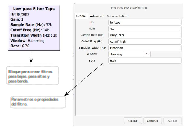
\includegraphics[width=.8\textwidth]{Modulaciones_digitales/lab21/pdf/lab21_1.pdf}
\end{figure}
\end{frame}
%*********************

\begin{frame}{Filter taps}
FIR Decimating
\begin{flushleft}
Este es un bloque que permite cargar toques de filtro desde un archivo (desde la herramienta de diseño de filtro).El nombre FIR viene de la manera en que el filtro afecta una señal. Una función impulso es una entrada bastante interesante, donde la señal es 0 siempre, excepto en un lugar donde tiene valor de 1.
\end{flushleft}
\end{frame}

%*********************

\begin{frame}{Filter taps}
\begin{figure}[H]
\centering
\vspace{-3mm}
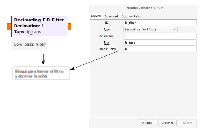
\includegraphics[width=\textwidth]{Modulaciones_digitales/lab21/pdf/lab21_2.pdf}
\end{figure}
\end{frame}

%*********************

\begin{frame}{Filter taps}
\begin{figure}[H]
\centering
\vspace{-3mm}
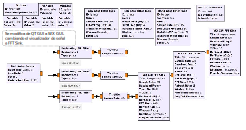
\includegraphics[width=\textwidth]{Modulaciones_digitales/lab21/pdf/lab21_3.pdf}
\end{figure}
\end{frame}
%*********************

\begin{frame}{Filter taps}
\begin{figure}[H]
\centering
\vspace{-3mm}
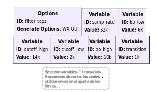
\includegraphics[width=\textwidth]{Modulaciones_digitales/lab21/pdf/lab21_4.pdf}
\end{figure}
\end{frame}

%*********************

\begin{frame}{Filter taps}
\begin{figure}[H]
\centering
\vspace{-3mm}
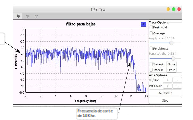
\includegraphics[width=\textwidth]{Modulaciones_digitales/lab21/pdf/lab21_5.pdf}
\end{figure}
\end{frame}

%*********************

\begin{frame}{Filter taps}
\begin{figure}[H]
\centering
\vspace{-3mm}
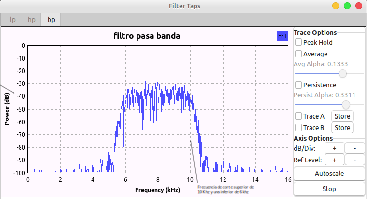
\includegraphics[width=\textwidth]{Modulaciones_digitales/lab21/pdf/lab21_6.pdf}
\end{figure}
\end{frame}





\subsection{Lab22: Python block}

%*********************
\begin{frame}{}

\pgfdeclareimage[width=\paperwidth,height=\paperheight]{bg}{imagenes/fondo_lab}
\setbeamertemplate{background}{\pgfuseimage{bg}}

\bfseries{\textrm{\LARGE Actividad\\ \Large Embedded Python Block}}
\raggedright
\end{frame}
%*********************

%--------------------------

\begin{frame}{Python block }


\pgfdeclareimage[width=\paperwidth,height=\paperheight]{bg}{imagenes/fondo3}
\setbeamertemplate{background}{\pgfuseimage{bg}}

  \begin{itemize}
  \item \justifying Le permite crear un nuevo bloque (personalizado) en Python sin necesidad de crear e instalar un Módulo fuera del árbol (OOT). Cuando agrega el bloque a su diagrama de flujo, el código rellenado previamente simplemente toma el flujo de entrada y lo multiplica por una constante. Tenga en cuenta que la estructura de este bloque de Python coincide con la estructura de un bloque de Python fuera del árbol (OOT) Es esencialmente un bloque Python OOT integrado en un diagrama de flujo grc.


 
  \end{itemize}
\end{frame}
%---------------------------

\begin{frame}{Python block}

\begin{figure}[H]
\centering
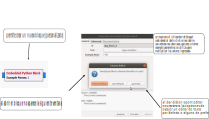
\includegraphics[width=\textwidth]{Modulaciones_digitales/lab22/pdf/lab22.pdf}
\end{figure}
\end{frame}
%--------------------


\begin{frame}{Python block }


\pgfdeclareimage[width=\paperwidth,height=\paperheight]{bg}{imagenes/fondo3}
\setbeamertemplate{background}{\pgfuseimage{bg}}

  \begin{itemize}
  \item \justifying Después de haber elegido nuestro editor por defecto o editor de texto preferente se nos genera un codigo del bloque. en el cual se ingresaran los parametros como se observara a continuacion en el ejemplo


 
  \end{itemize}
\end{frame}
%---------------------------

\begin{frame}{Python block}
\vspace{-1cm}
\begin{figure}[H]
\centering
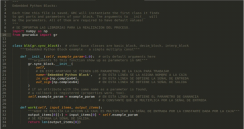
\includegraphics[width=1.1\textwidth]{Modulaciones_digitales/lab22/pdf/lab22_1.pdf}
\end{figure}
\end{frame}
%_---------------------

\begin{frame}{Python block}
\vspace{-1.5cm}
\begin{figure}[H]
\centering
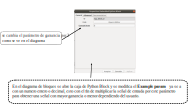
\includegraphics[width=1.1\textwidth]{Modulaciones_digitales/lab22/pdf/lab22_2.pdf}
\end{figure}
\end{frame}
%_---------------------
%_---------------------

\begin{frame}{Python block}
\vspace{-1.5cm}
\begin{figure}[H]
\centering
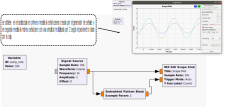
\includegraphics[width=1.1\textwidth]{Modulaciones_digitales/lab22/pdf/lab22_3.pdf}
\end{figure}
\end{frame}
%_---------------------

%///////////////////////////////////////////////////////////////



%/////////////////////////
\section{BIBLIOGRAFÍA}
\begin{frame}

\pgfdeclareimage[width=\paperwidth,height=\paperheight]{bg}{imagenes/fondo_seccion}
\setbeamertemplate{background}{\pgfuseimage{bg}}

\definecolor{greenU}{RGB}{212,202,72}
\setbeamercolor{block body}{fg=Black,bg=greenU}
\begin{block}{}
\centering
\vspace{8mm}
\Large{BIBLIOGRAFÍA}
\vspace{8mm}
\end{block}
\end{frame}
%-----------------------

\begin{frame}[allowframebreaks]
\frametitle{Referencias}

\pgfdeclareimage[width=\paperwidth,height=\paperheight]{bg}{imagenes/fondo3}
\setbeamertemplate{background}{\pgfuseimage{bg}}

\bibliographystyle{unsrt}
\begin{thebibliography}{11}







%-----
\bibitem{Seeber2014} Seeber, Balint.
\newblock "GNU Radio Tutorials Labs 1 – 5". [Online] \url{https://files.ettus.com/tutorials/labs/Lab\_1-5.pdf}. 

%-----
\bibitem{Conferencia2015} Vachhani, Khyati. Gokhruwala, Kenil; Kumar, Jay  
\newblock "Design Analysis of Digital Modulation Schemes with GNU Radio". [Descargado de:] \url{https://www.researchgate.net/publication/281106848_Design_Analysis_of_Digital_Modulation_Schemes_with_GNU_Radio}. 

%-----
\bibitem{Wikipedia8} Wikipedia.
\newblock "Frecuencia modulada". [Online] \url{https://es.wikipedia.org/wiki/Frecuencia_modulada}. 

%-----
\bibitem{linuxjournal1995} Vaught, Andy.
\newblock "Introduction to Named Pipes". [Online] \url{https://www.linuxjournal.com/article/2156}. 

%-----
\bibitem{wikiopendigital} Wiki Opendigitalradio.
\newblock "Simple FM transmitter using gnuradio". [Online] \url{http://wiki.opendigitalradio.org/Simple_FM_transmitter_using_gnuradio}. 

%-----

\bibitem{FichaTecnica} Electronisys.
\newblock "Ficha técnica de radio portátil UHF Motorola EP150". [Descargado de:] \url{http://www.electronisys.cl/index.php?route=product/product&product\_id=50}. 

%-----
\bibitem{Wikipedia2018} Wikipedia.
\newblock "Continuous Tone-Coded Squelch System". [Online] \url{https://en.wikipedia.org/wiki/Continuous\_Tone-Coded\_Squelch\_System}. 

%-----
\bibitem{Airspy2018} Airspy.
\newblock "Airspy Redefining the Radio Experience". [Online] \url{https://airspy.com/download/}

%-----
\bibitem{Motorola2010} Motorola Solutions.
\newblock "Two-Way Radios". [Online] \url{https://www.motorolasolutions.com/content/dam/msi/docs/enxl/products/two-way-radios-business/portable-radios/on-site-smallbusiness/}. 

%-----
\bibitem{Lecture9} Documento PDF
\newblock "Lecture 9 Analog and Digital I/Q Modulation". [Online] \url{http://web.mit.edu/6.02/www/f2006/handouts/Lec9.pdf}.

%-----

\bibitem{Institute of  Technology} TOMASI, WAYNE.
\newblock "Sistemas de comunicaciones electrónicas". [Descargado de:] \url{http://fernandoarciniega.com/books/sistemas-de-comunicaciones-electronicas-tomasi-4ta-edicion.pdf}.
%-----

\bibitem{Universidad Militar Nueva Granada} Arévalo Nelson
\newblock "Transmisión y recepción de imagen con modulación QPSK usando radio definido por software". [Online] \url{https://repository.unimilitar.edu.co/handle/10654/16606}. 
%-------------------------------------------------------------------------------------
\bibitem{Oregon Institute of Technology} Aaron Scher 
\newblock "Cómo convertir un flujo de datos digitales en una señal analógica de banda base utilizando un filtro FIR interpolador". [Online] \url{hhttp://aaronscher.com/GNU_Radio_Companion_Collection/BPSK_modulatorB.html}. 
%------------------------------------------------------------------------------------
\bibitem{Navipedia 2011} Agencia Nacional Europea
\newblock "Señales de coseno realzado de raíz cuadrada ". [Online] \url{https://gssc.esa.int/navipedia/index.php/Square-Root_Raised_Cosine_Signals_(SRRC)/tutorials/labs/Lab\_1-5.pdf}. 

\end{thebibliography}


\end{frame}

%/////////////////////////

%\input{soluciones/soluciones}




\end{document}
